\chapter{ Metodologia}\label{meto}


\section{ Metodologia utilizada}\label{intro:metodologia}

O objetivo deste projeto é propor um Modelo preditivo de Suporte à Decisão que dê apoio a um gestor quando decidir enviar uma frota de 
caminhões por determinada rodovia que apresente retenções crescentes de logística de cargas.\\

Dados governamentais tais como PRF, INPE, IBGE são iniciativas governamentais para fomentar a participação popular, também é 
conhecido como \textit{Open data} \cite{DadosGoverno}, contudo os dados referentes à PRF e ao BPRv foram cedidos pelos respectivos 
órgãos governamentais para serem utilizados exclusivamente nesta pesquisa.

Para isso montarmos o modelo preditivo utilizamos bases de dados históricas da PRF (de acidentes e de paralisações ex: protestos), bases de dados
do Batalhão de Polícia de Rodoviária estadual -- BPRv, bases de dados do INPE e base de dados do IBGE. Todas essas bases de dados são integradas
gerando um único e complexo modelo preditivo que é acoplado a estrutura dinâmica.

A estrutura dinâmica é composta por duas API's, uma disponibilizada pelo Google Maps que está atualmente na versão V3 e outra uma API do Twitter,
que proporciona uma ``leitura'' atualizada em forma de mapa no momento em que o sistema ``roda''. 
A API do Twitter também tem a possibilidade de atualizar o modelo preditivo, fazendo um Arco cibernético, retroalimentando todo o sistema. 
Isso permite que o primeiro módulo (preditivo) seja atualizado de tempos em tempos.

A API Google Maps portanto é o ``front-end'' do Sistema e uma futura aplicação que poderá ser desenvolvida para ser executada em um aparelho 
celular, ``Smartphones'', com boa capacidade para executar aplicativos mais complexos.

\pagebreak

\section{ Reflexão sobre as tecnologias utilizadas no modelo preditivo}\label{result}

Não existe uma técnica de mineração que generalize os mais diversos ambientes preditivos, mas sim um ``pool'' dessas técnicas onde uma complementa outra.
As técnicas preditivas tradicionais que contemplam análise de grandes massas de dados como base heterogêneas são possíveis quando adaptadas para uma forma comparável à que
foram inicialmente concebidas. Algumas técnicas de IA são altamente sensíveis a dados ausentes os ``missing data'' à dados com pouca consistência e outros tipos de dados 
comuns em bases mantidas sem um bom critério de inserção dos dados. Nesta pesquisa, bases heterogêneas foram integralizadas num única grande base, onde as variáveis independentes foram
em sua maioria preservadas e/ou construídas novas, nas bases onde não haviam correspondência, respeitando a lógica do negócio. 
A variável dependente foi designada como \textbf{gargalo} e as variáveis independentes (ou explicativas) são:

\begin{table}[htbp]
 %\centering
  \caption{Variáveis do modelo preditivo}
  
  \begin{tabular}{r|l} \hline
   KM & Numeração do quilômetro \\
    BR & Numeração da Br\\
    condPista & Condição da pista: seca, molhado, ... \\
    restVisibili & Restrição de visibilidade: inexistente, neblina, .., outros \\
    tipoAcident & Tipo de Acidente: atropelamento, colisão, paralisação,...\\
    tipoDano  & Tipo de Dano: leve, médio, grave \\
    Municipio  & Localidade onde ocorreu \\
    Ano & Ano que ocorreu o acidente \\
    Mês & Mês que ocorreu o acidente \\
    Dia & Dia que ocorreu o acidente \\
    Hora & Hora que ocorreu o acidente \\
  \end{tabular}
\end{table}

 
A base de dados da PRF, relativas a paralisações das vias, por motivos diversos, não haviam variáveis tais como (visibilidade, condições da via, gravidade paralisação e outras).
Presumivelmente protestos são realizados com boa visibiliade, em condições de via rezoáveis e a gravidade da paralisação foi considerada leve.

As técnicas como Redes Neurais Artificias (MLP), Árvores de decisão (CART), Regressão logística (MLR) nos forneçam uma
visão generalizada dos fatores preponderantes quando os dados estão tratados.

\begin{itemize}
 \item[a] Redes Neurais Artificias do tipo \textit{ Multi Layer Perceptron}  -- (MLP) têm capacidade de receber várias entradas ao mesmo tempo e distribuí-las de maneira organizada, além 
	  são simples de implementar e trazem resultados satisfatórios em grandes bases de dados.
 
 \item[b] Árvores de decisão para classificar acidentes do tipo \textit{ Classification and Regression Tree}  -- (CART) foi empregue por Pakgohar et al no artigo 
	  \textit{The role of human factor in incident and severity of road crashes based on the CART and LR regression a data mining approach}  com nível de acurácia próximo aos 80\%

 \item[c] Regressão logística tipo \textit{Multinomial Logistic Regression} -- (MLR) fornece a possibilidade de aprofundamento em vários níveis de busca sendo a mais apropriada, já que Regressão logística 
	  tradicional não permite aprofundamento desse tipo no espaço de busca.
\end{itemize}



Propomos um plano que contemple 3 etapas, cada uma dividida em fases atinentes. A figura 3.1 ilustra essa metodologia descrita graficamente, onde as três etapas são representadas por retângulos.
 
\begin{figure}[ht]
\centering
\caption{Etapas da metodologia}
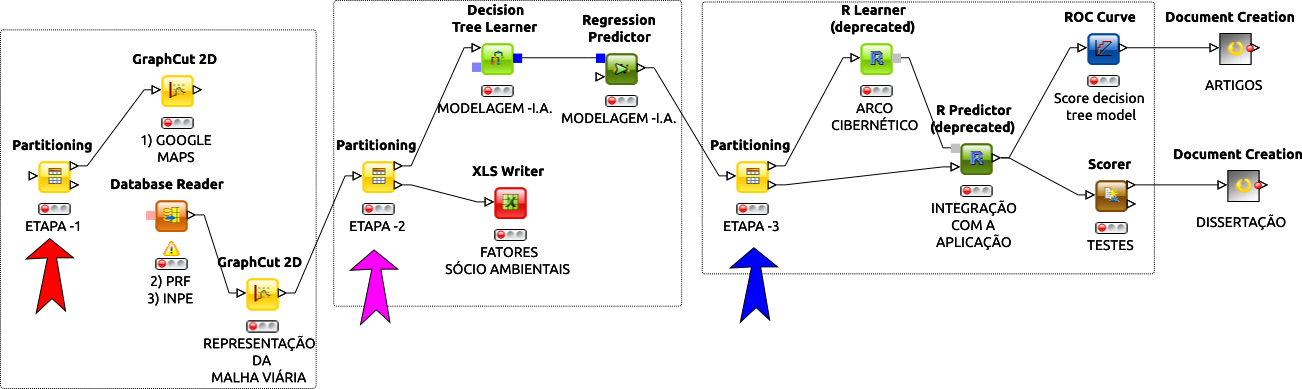
\includegraphics[width=150mm, height=60mm]{Figuras/BigData/Etapas.png}
\end{figure}

 

 \pagebreak
 O retângulo da esquerda é a etapa 1, onde há a representação da malha viária.
 A etapa 1 contempla as fases da coleta das bases vetoriais, das bases de dados históricas e proposição de um modelo de representação único.
 
 O retângulo central é a etapa 2, que consiste nas fases de Identificação dos fatores sócio ambientais na bases históricas, a modelagem do sistema preditivo e aplicação das técnicas de IA. Propomos inicialmente a Regressão Logística e Árvores de decisão, testes iniciais e depuração do modelo.
 
 A última etapa da nossa proposta metodológica é a etapa 3, esta conterá um arco cibernético construído com os dados de redes sociais, como por exemplo a API do Twitter, este ``per si'' fará com que o modelo preditivo seja retro-alimentado, 
 mantendo-o, ao longo do tempo atualizado na perspectiva do usuário gestor. Isso pois, modelos preditivos com o passar do tempo tendem a desfasar-se. Uma proposta algorítmica para substituir a API das redes sociais 
 poderá ser desenvolvida e testada numa fase complementar, o algorítmo Ant-Miner poderá vir a ser um candidato de adaptação.
 
 Concluída as três etapas e com as informações geradas pelo modelo serão escritos artigos científicos  pertinentes à pesquisa em lide e a escrita da dissertação.
 
 
 
 
\section{Cronograma}\label{intro:cronograma}


\begin{table}[htbp]
 \scriptsize
      \centering  \caption{Cronograma -- 12 meses}
	\begin{tabular}{l|c|c|c|c|c|c|c|c|c|c|c|c}
	\hline
	\textbf{Etapas/2016} & \textbf{Fev} & \textbf{Mar} & \textbf{Abr} & \textbf{Mai}& \textbf{Jun} & \textbf{Jul} & \textbf{Ago} & \textbf{Set} & \textbf{Out} & \textbf{Nov} & \textbf{Dez} & \textbf{Jan/17} \\
	  \hline
	  Rev. da literatura. & x & x & x & x & x & x & x & --- & --- & --- & --- & --- \\ \hline
	  Etapa -- 1 & x & x & x & --- & --- & --- & --- & --- & --- & --- & --- & --- \\ \hline
	  Etapa -- 2 & --- & --- & --- & x & x & x & --- & --- & --- & --- & --- & --- \\ \hline
	  Etapa -- 3 & --- & --- & --- & --- & --- & --- & x & x & x & --- & --- & --- \\ \hline
	  Escrita de artigos & --- & --- & --- & --- & --- & --- & --- & --- & x & x & x & --- \\ \hline
	  Escrita da dissertação & --- & --- & --- & --- & --- & --- & --- & --- & x & x & x & --- \\ \hline
	  Defesa & --- & --- & --- & --- & --- & --- & --- & --- & --- & --- & --- & x \\ \hline
	\end{tabular}
\end{table}


 



